%% ----------------------------------------------------------------
%% Analysis.tex
%% ---------------------------------------------------------------- 


\chapter{Analysis of Purposive Social Network} \label{Chapter: Analysis of Purposive Social Network}

A purposive social network is a broad and general concept that can be applied to many different social networks. At its core, it is a network with a specific goal and purpose where people come together to solve a particular problem.

For this research StackOverflow website is analyzed where programmers and developers ask questions and experts in the field answer them and solve the problem. In this analysis, the user asking and answering questions, voting the responses and commenting are the main entities of the social network. Their network ties are measured by their communication and interaction between them. The amount of their contribution is measured by the crowdsourcing where people give up votes or down votes to their posts and the badges they receive for their contribution.

\section{Network Linkage and Social Ties}

StackOverflow is not a typical social networking website per se as users cannot create an explicit friendship or follow other people�s work, they cannot send private messages or form groups.

The social ties are form implicit by user interaction with each other through asking questions and answering them, voting on the posts and commenting on them. The communication network is studied to see the social ties of the individuals \cite{monge2003theories}.

\begin{table}[!htb]
  \centering
  \begin{tabular}{cc}
  \toprule
  \textbf{Post Type} & \textbf{Number}\\
  \midrule
   Questions & 3279233\\   \midrule
   Answers & 6578079\\   \midrule
   Registered Users & 1225580\\   \midrule
   Tags & 30408 \\   \midrule
   Unanswered Questions & 780535\\   \midrule
   Badges & 3454994\\   \midrule
   Votes & 26184363\\   \midrule
   Comments & 12526162\\ 
  \bottomrule
  \end{tabular}
  \caption{StackOverflow at glance as of June 2012}
  \label{Table:tabex}
\end{table}

As of June 2012, there are over one million registered users in StackOverflow and more than 3.2 millions questions asked by users. The questions are categorized using tags and individual users can subscribe to tags to receive daily email of all the question asked in the tag. There are more than 30 thousand tags associated with various questions and answers. Users have casted more than 26 million votes to mark the good questions and answers.

\begin{figure}[!htb]
  \centering
  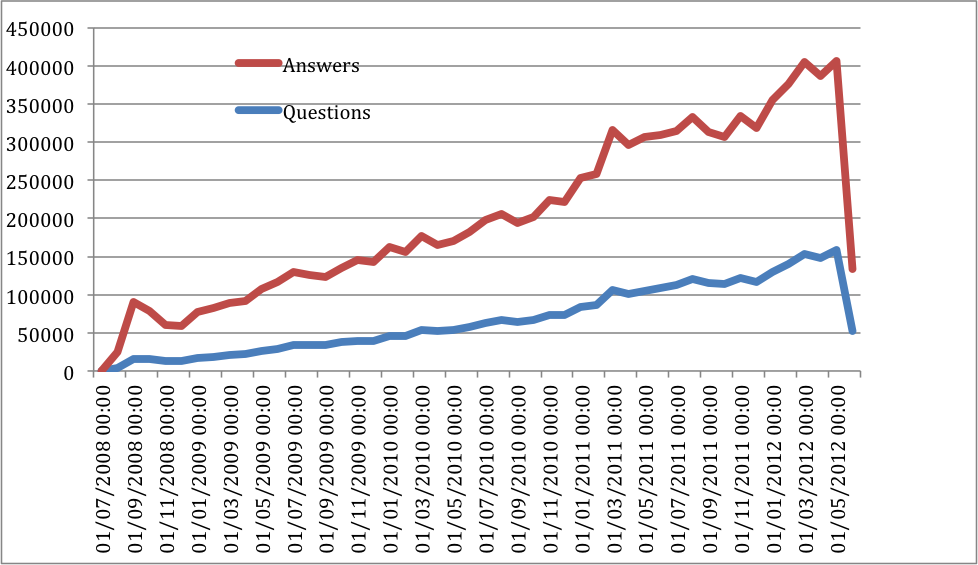
\includegraphics[width=15cm]{qa.png}
  \caption{Questions and answers posted per month on StackOverflow}
  \label{Figure:figex4a}
\end{figure}

The \fref{Figure:figex4a} shows the number of questions asked and answered by users each month. In the year 2012, each questions have on average 1.645 number of answers.

This community is made of programmers and their motivation is to solve the problem they had encountered and to provide answers to gain reputations. Thousands of questions and answers are posted everyday. The analysis of posts shows that the programmers prefer to ask the questions and answers on weekdays.

\begin{figure}[!htb]
  \centering
  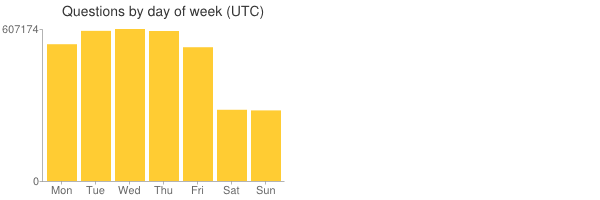
\includegraphics[width=15cm]{chart1.png}
  \caption{Questions posted by the day of week}
  \label{Figure:figex4b}
\end{figure}

Despite high user feedback and participation, 23.79\% of questions are not answered or the answers do not receive any up votes. On average a question receives 2.006 answers and .12\% of questions receives more than 15 answers.

\begin{figure}[!htb]
  \centering
  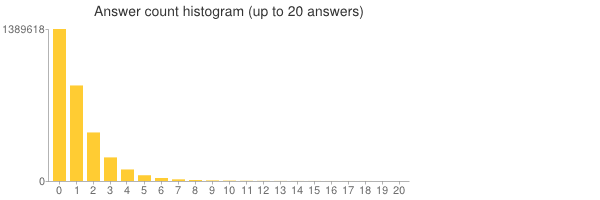
\includegraphics[width=15cm]{chart2.png}
  \caption{Answer count to the questions}
  \label{Figure:figex4c}
\end{figure}

The questions are answers are provided with tags to categorize and arrange for easy search and discovery. The entire website is categorized using the tags and the list of most popular tags are shown in the table. The figure shows the weekly use of the popular tags. The number of questions asked for each tags also provides an insight on the popular language used by developers at the time.

\begin{table}[!htb]
  \centering
  \begin{tabular}{cc}
  \toprule
  \textbf{Tags} & \textbf{Number of instance}\\  \midrule
   C\# & 370074 \\ \midrule
   JAVA &  315488 \\ \midrule
   PHP & 293755 \\ \midrule
   JavaScript & 278592 \\ \midrule
   Android & 244791 \\
  \bottomrule
  \end{tabular}
  \caption{Five most popular tags and its instances}
  \label{Table:tabex2}
\end{table}

\begin{figure}[!htb]
  \centering
  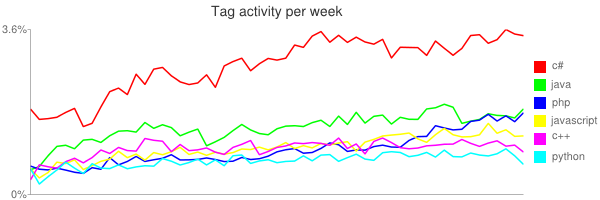
\includegraphics[width=15cm]{chart3.png}
  \caption{Tag trends per week of most popular tags}
  \label{Figure:figex4d}
\end{figure}

The analysis of questions shows that each question has between one to five tags associated with it. Most questions (70.30\%) have 2 to 4 tags associated with it. The relationship between the tags shows the overlapping of networks and how it is tied with one another.

\cite{Eberhardt2012} provided an interactive graph in his website to show the relationships between the most popular tags and how closely they are related to each other. In the following graph each segment size is directly proportional to the number of instance it is used and the connection between the tags indicate the times they have been used together in a question. The thickness of the connection shows the strength of the relations. The segment is colour coded by the frequency of connections, red segments are strongly connected and blue segments are weakly connected.

\begin{figure}[!htb]
  \centering
  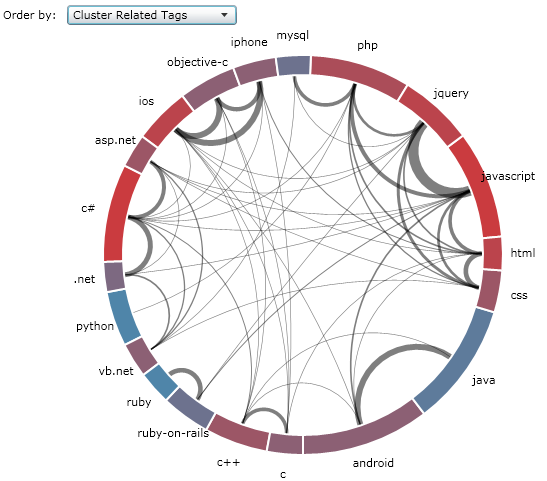
\includegraphics[width=11cm]{graph1.png}
  \caption{Related tags clustered together}
  \label{Figure:figex4e}
\end{figure}

\begin{figure}[!htb]
  \centering
  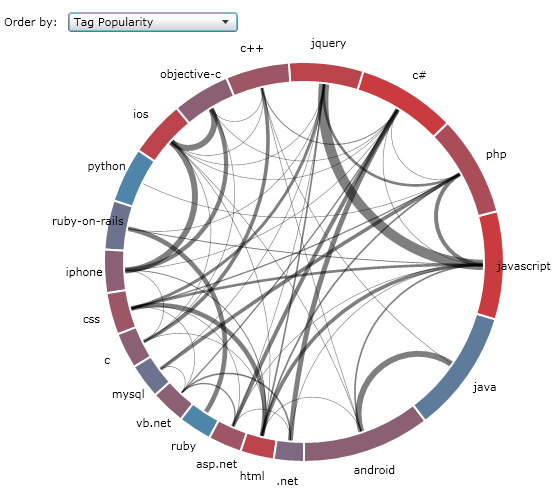
\includegraphics[width=11cm]{graph2.png}
  \caption{Popular tags clustered together}
  \label{Figure:figex4f}
\end{figure}

The clustering of the tags shows the relationship between the tags and technologies. The two popular tags JAVA and Android are closely related to each other but are scarcely joined with other tags. The strongest relationship is between jQuery and JavaScript because the overlapping framework of the two programming languages. C, C++ and C\# are also a closely related groups as well as iOS, Objective-C and iPhone. However, sometimes Objective-C is also tagged with C, C++ and C\#, if by mistake or deliberately can be argued.
There is a large cluster of connected web development languages, CSS, HTML, JavaScript and jQuery, indicating the close knit use of these technologies in development of website and web applications. The interesting thing is the relationship between the scripting langue PHP and Python, they are popular tags but are sparsely connected with other tags and are weakly linked with database related tags.

\section{Role of Individual Actors}

Users who contribute to the website are the main actors of this purposive social network. There are more than 1.2 million registered users in StackOverflow and they ask the questions, answer it, vote it and moderate the community. The users are not directly linked to each other to create relationships; in this network the relationship is formed by their interaction and their contribution. The user behaviour, their motivation to use the website and incentive to contribute is described below.

Despite the high content generation by the users, 56.02\% do not interact or contribute to the website, they have 1 reputation point that they receive while joining the website.

\begin{figure}[!htb]
  \centering
  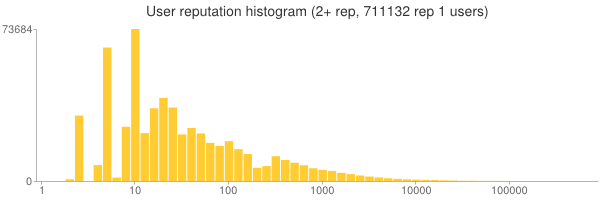
\includegraphics[width=15cm]{chart4.png}
  \caption{User reputation histogram}
  \label{Figure:figex4g}
\end{figure}

\begin{table}[!htb]
  \centering
  \begin{tabular}{cc}
  \toprule
  \textbf{Reputation} & \textbf{Number of users}\\  \midrule
  1 & 669554\\ \midrule
  2-10 & 126235\\ \midrule
  11-100 & 295389\\ \midrule
  101-1000 & 3161130\\  \midrule
  1001-10000 & 170993\\ \midrule
  10001-20000 & 1437\\ \midrule
  20001-100000 & 895\\ \midrule
  100001-200000 & 49\\ \midrule
  less than 200000 & 11\\
  \bottomrule
  \end{tabular}
  \caption{Number of users with reputations}
  \label{Table:tabex3}
\end{table}

As \tref{Table:tabex3} shows, there are 669554 users with 1 reputation point and one user with 452951 reputation points. The distribution of the users reputation shows that more than half of the users are lurkers and the elite users with the most reputation points are the editors and moderators of the community and are considered the expert in their field.

The reputation of the user has a direct correlation with the trust in the community. StackOverflow has designed an excellent reward program to motivate and incentivize the users to contribute and gain more reputations and badges.

Currently, there are 77 different types of badges given to the user based on their contribution. There are badges given to the user who asks questions with 1 reputation point (Student), to the user who edits the answers to make posts better (Editor) and to even an active user for a year (Yearling). This type of virtual acknowledgement of efforts encourage the user to participate and contribute to the website.

The other method that encourages the users to participate is the promptness of the response. The asker prefers to receive information sooner rather than later, and will stop the process when satisfied with the cumulative value of the posted information. The analysis of the posts shows that half of the questions get an answer within an hour of the posting and within a day the questions receives an accepted answer. When the answers are delayed, the questioners look for alternative websites to get a response.

\begin{figure}[!htb]
  \centering
  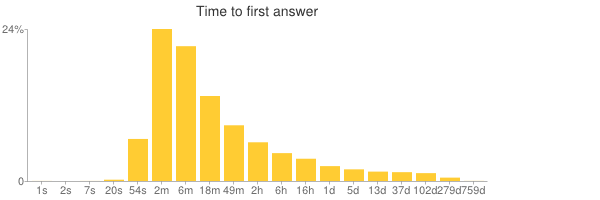
\includegraphics[width=15cm]{chart5.png}
  \caption{Time to receive the first answer}
  \label{Figure:figex4h}
\end{figure}

\begin{figure}[!htb]
  \centering
  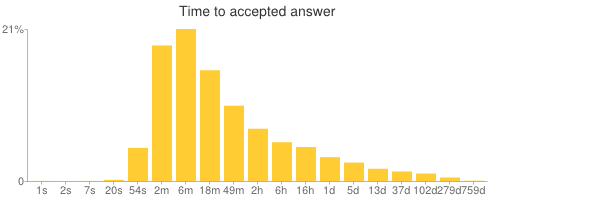
\includegraphics[width=15cm]{chart6.png}
  \caption{Time to get the accepted answer}
  \label{Figure:figex4i}
\end{figure}

\section{Incentive Design and Quality Control}

The StackOverflow website uses a game theoretic model to encourage user participation and activity. Participation is encouraged through an elaborate point system and users also receive badges for participation. Also, the top contributor and user with highest reputation are featured on the question page, giving the user more visibility and acknowledgement of the user�s expertise. This encourages participants to accumulate more points and contribute to get recognition.

When an answer is votes up, the user gains 10 reputations and 5 points when the question is voted up. When an answer is accepted the user receives 15 points and there is also negative point system, a user looses 2 reputation point when a question or an answer is voted down. This keeps the spamming in check and repeated questions and answers are avoided.

The system also encourages users to participate as the higher reputation points gain more privileges. When a user has 15 reputation points, only then they can up vote and 50 points allows users to comment. To stop harassment and spam, user requires 125 reputation points to vote down and it costs the user 1 reputation point. The incentive model is thorough and higher reputation points open more gates for users to interact and contribute and be acknowledged as the expert in their field.

The community thrives because of the high quality of content and it is possible by the user�s action and moderation. Users vote up the good questions and answers and vote down the bad quality content or repeated posts. There is more than 6 million votes casted in the website and the user with enough reputations are allowed to cast 40 votes per day.

\begin{figure}[!htb]
  \centering
  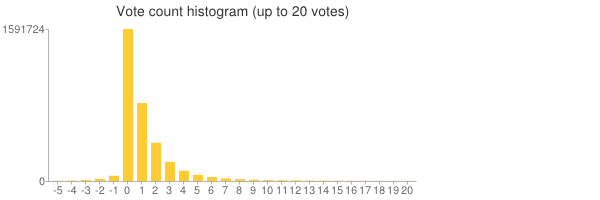
\includegraphics[width=15cm]{chart7.png}
  \caption{Vote count histogram}
  \label{Figure:figex4j}
\end{figure}

\begin{table}[!htb]
  \centering
  \begin{tabular}{cc}
  \toprule
  \textbf{Vote} & \textbf{Vote Count}\\  \midrule
  less than 20 & 25\\  \midrule
  0 & 504754\\  \midrule
  1-10 & 7802690\\  \midrule
  11-100 & 718650\\  \midrule
  101-1000 & 6460\\  \midrule
  1000-5000 &11\\
  \bottomrule
  \end{tabular}
  \caption{Questions� votes count}
  \label{Table:tabex4}
\end{table}

The analysis of the questions and votes shows that every question receives 3.06 votes on average. One question received negative 115 votes and the highest vote received to a question is 2499. Similar analysis of answers and their votes shows that, on average an answer receives 0.99 votes and the lowest vote to an answer is negative 57 and the highest vote is 4432.

\section{Using Semantic Web Technologies}

The data extracted from StackOverflow website is in the form of simple text, some of the posts contain HTML codes but they are snippets of code and are represented as text in the database. The users categorize the posts by using tags and it gives information about the topic and the programming language the question is being asked. The answers do not have special tags but the tags of the questions are applied to the answers as well.

\subsection{Using RDF and Linked Data}

All the user data, post data, votes and badges are transformed in RDF data by applying simple RDF schema and ontologies.

The website only shows basic user profile information due to the privacy reasons and FOAF ontology is used to describe the data. An example of the simple user profile information is as follows:

\begin{verbatim}
<foaf:Person>
    <foaf:name> Geoff Dalgas </foaf:name>
    <foaf:mbox_sha1sum> b437f461b3fd27387c5d8ab47a293d35 </foaf:mbox_sha1sum>
    <foaf:based_near> Corvallis, OR </foaf:based_near>
    <foaf:age> 35 </foaf:age>
    <foaf:OnlineAccount> http://stackoverflow.com/users/2/geoff-dalgas 
    </foaf:OnlineAccount
</foaf:Person>
 \end{verbatim}
 
 Similarly, the posts created by users, the questions and answers are described using SIOC ontology. The content is described and linked with the user RDF using the similar URIs.
 
\begin{verbatim}
<sioc:Post rdf:about=" http://stackoverflow.com/questions/89228/calling-an-external
-command-in-python">
    <dcterms:title>Calling an external command in Python</dcterms:title>
    <dcterms:created> 2008-09-18T21:42:52.667 </dcterms:created>
    <sioc:has_container rdf:resource=" http://stackoverflow.com/questions/tagged
    /python"/>
    <sioc:has_creator>
       <sioc:UserAccount rdf:about=" http://stackoverflow.com/users/170339/bludger " 
       rdfs:label="bludger"> </sioc:UserAccount>
     </sioc:has_creator>
     <sioc:content>How can I call an external command in Python</sioc:content>
     <sioc:topic rdfs:label="python" rdf:resource=" http://stackoverflow.com
       /questions/tagged/python"/>
     <sioc:topic rdfs:label="command" rdf:resource=" http://stackoverflow.com
       /questions/tagged/command"/>
     <sioc:has_reply>
        <sioc:Post rdf:about=" http://stackoverflow.com/a/89243/1313327">
            <sioc:content>Look at the subprocess module in the stdlib: from subprocess 
             import call call(["ls", "-l"]) The advantage of subprocess vs system is that 
             it is more flexible (you can get the stdout, stderr, the "real" status code, 
             better error handling, etc...). I think os.system is deprecated, too, or will
             be: http://docs.python.org/library/subprocess.html#replacing-older-functions
             -with-the-subprocess-module For quick/dirty/one time scripts, os.system
             is enough, though.</sioc:content>
             <dcterms:created>2008-09-18T23:42:52.667</dcterms:created>
             <sioc:has_creator>
                <sioc:UserAccount rdf:about=" http://stackoverflow.com/users/11465
                 /david-cournapeau" rdfs:label=" david-cournapeau "> </sioc:UserAccount>
              </sioc:has_creator>
           </sioc:Post>
      </sioc:has_reply>
</sioc:Post>
\end{verbatim}

\subsection{Topic Disambiguation}

The StackOverflow dataset is sparsely annotated by user-generated tags and it is not linked with any other datasets. When user creates a question, they add tags to it to categorize into different topics but the answers have the tags from the questions. Also, all the main topics inside the text of question or answer is not clearly stated. The topics are ambiguous and not linked to any vocabulary or properly annotated.

A sample of the question, answer and tag data is annotated with the links from Wikipedia datasets and Drupal datasets to resolve the name and topic disambiguation. These services do the name entity recognition and match the entities with the appropriate topics and categories. The service does not convert the text into Linked Data or RDF, the returned data is further transformed into RDF and linked with the DBpedia dataset.

Wikipedia Miner service is used to annotate a small sample of posts, the service returns the text with annotated topics embedded into the text. The service accepts simple text or HTML and one can specify the density of links to be added and the level of accuracy required from the service. Below is an example annotated text of a question and answer posted.

\begin{figure}[!htb]
  \centering
  \subfigure[Annotating a text question]{
    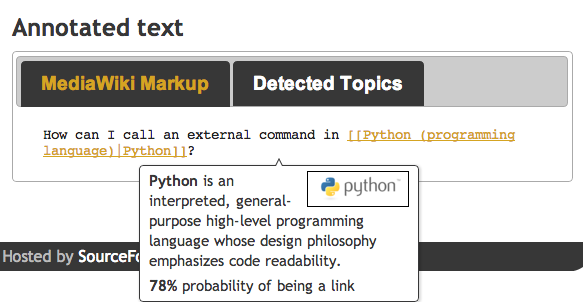
\includegraphics[width=14cm]{q.png}
    \label{Figure:figsubex11:left}
  }
  \subfigure[Annotating a text answer]{
    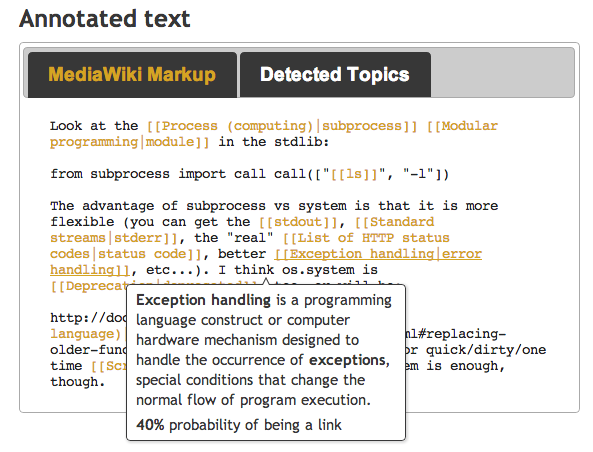
\includegraphics[width=14cm]{ans.png}
    \label{Figure:figsubex11:right}
  }
  \caption{Wikipedia Miner web service annotating a text question and an answer}
  \label{Figure:figsubex11}
\end{figure}

The Wikipedia miner service uses a word sense disambiguation based machine learning algorithm and where it detects key terms in a text excerpt and disambiguating then against Wikipedia article. It provides a JAVA API to access the Wikipedia database, including all the categories and it can be searched, browsed and iterated over \cite{milne2012open}.

OpenCalais is another web service used to annotate the StackOverflow posts with the Drupal dataset. This tool creates a semantic rich metadata for the content using the natural language processing, machine learning and name disambiguation algorithm. It provides many services; it provides tag integration with different taxonomy and vocabulary, geo-mapping of location and semantic annotation of keywords. An example annotation of text using OpenCalais is below.

Text sample question: "Does Python have a ternary conditional operator? If not available, is it possible to simulate one concisely using other language constructs?"

\begin{verbatim}
<SocialTags>
  <SocialTag importance="2"> Conditional
	<originalValue>Conditional (programming)</originalValue>
  </SocialTag>
  <SocialTag importance="2"> Python
  	<originalValue>Python (programming language)</originalValue>
  </SocialTag>
  <SocialTag importance="2"> C
  	<originalValue>C (programming language)</originalValue>
  </SocialTag>
  <SocialTag importance="2"> Ternary operation
  	<originalValue>Ternary operation</originalValue>
  </SocialTag>
  <SocialTag importance="1"> Software engineering
  	<originalValue>Software engineering</originalValue>
  </SocialTag>
  <SocialTag importance="1"> Computing
  	<originalValue>Computing</originalValue>
  </SocialTag>
  <SocialTag importance="1"> Computer programming
  	<originalValue>Computer programming</originalValue>
  </SocialTag>
</SocialTags>
\end{verbatim}

As seen from above snippet, the OpenCalais service finds the keywords and matches it with a taxonomy or vocabulary and assigns the importance to the tag that it is disambiguating.

Both the services do the name entity recognition and match it to a known vocabulary and taxonomy. They do a natural language processing of the text and annotate the keywords. This annotation is then matched with the Wikipedia topics and the StackOverflow data is linked to the Wikipedia data.

These links when analyzed tell the type of categories the keywords matched to give additional information that the StackOverflow tags do not provide. The analysis shows the most asked question is asked from the following categories of programming languages:

\begin{table}[!htb]
  \centering
  \begin{tabular}{cc}
  \toprule
  \textbf{Annotated keyword} & \textbf{StackOverflow Tags}\\  \midrule
  Programming Language & C\#, JAVA, Python\\ \midrule
  Framework & jQuery, ASP.net\\ \midrule
  Environment & Android, iPhone\\ \midrule
  Database & MySQL, SQLite\\
  \bottomrule
  \end{tabular}
  \caption{Keyword analysis of StackOverflow question tags}
  \label{Table:tabex5}
\end{table}

It can be seen from the above example, name entity recognition, creating vocabulary and matching the keywords to a topic and linking it to another knowledgebase provides additional information. This leads to better search and discovery of information and using this an expert in a particular field can also be determined. JAVA being a programming language is also an Object Oriented language and the expert of JAVA also has a good grasp of Object Oriented programming concept and hence can help users in both the scenario.

\subsection{Expert Finder}

According to the StackOverflow website the top user or an expert of C\# is Jon Skeet with more than eighty thousand reputation points and Python is Alex Martelli with more than nineteen thousand reputation point. These users appear on the individual pages of the tags as the top users and without the tag disambiguation they only appear as an expert on a particulate tag, not the joint concept of the topic.

\begin{table}[!htb]
  \centering
  \begin{tabular}{cc}
  \toprule
  \textbf{Tag} & \textbf{Top User with reputation point}\\  \midrule
  C\# & Jon Skeet (80.6k)\\ \midrule
  Java & Jon Skeet (39.7k)\\ \midrule
  Python & Alex Martelli (19.8k)\\ \midrule
  PHP & Pekka (9k)\\ \midrule
  Javascript & CMS (12.3k)\\ 
  \bottomrule
  \end{tabular}
  \caption{Top users of top tags in StackOverflow}
  \label{Table:tabex6}
\end{table}

When the tags are disambiguated and the keywords are matched to the topics, both Java and C\# is categorized at the Object Oriented programming language and here Jon Skeet is considered as an expert in the whole area with more than one hundred and twenty thousand reputation points. Similarly, when the programming languages are further categorized as server side script ion language with Python, PHP and Perl as main languages, Alex Martelli is considered as an expert and the user CMS is expert in the clients side languages such as Java and AJX with twelve thousand reputation points.

\begin{table}[!htb]
  \centering
  \begin{tabular}{cc}
  \toprule
  \textbf{Disambiguated Keywords} & \textbf{Top User with reputation point}\\  \midrule
  Object Oriented programming (C\#, Java) & Jon Skeet (120.3k)\\ \midrule
  Programming language(C\#, Java, Python) & Jon Skeet (120.7k)\\ \midrule
  Server side Scripting language (Python, PHP, Perl) & Alex Martelli (20.2k)\\ \midrule
  Clientside Scripting language (Javascript, AJAX) & CMS (12.3k)\\ 
  \bottomrule
  \end{tabular}
  \caption{Top users of top disambiguated topics in StackOverflow}
  \label{Table:tabex7}
\end{table}

Semantic web and linked data helped in topic  recognition and disambiguation and experts in broader concept and also specialized field can be ascertained even though these information is not present in the main website. The \tref{Table:tabex7} only shows the experts in StackOverflow domain, when the data from multiple website and question/answer forums are combined, the linked data can help find experts in across domain in bigger set of users and help in better search and discovery of experts and information.